\documentclass{article}
\usepackage{tikz}
\usetikzlibrary{knots}

\tikzset{
  basic strand/.style={
    red,
    line width=2pt,
    double=white,
    double distance=9pt,
  },
  crossing strand/.style={
    line width=13pt,
    only when rendering/.style={%
      draw=white,%
      line width=9pt,
      double=none,
    }
  }
}

\begin{document}

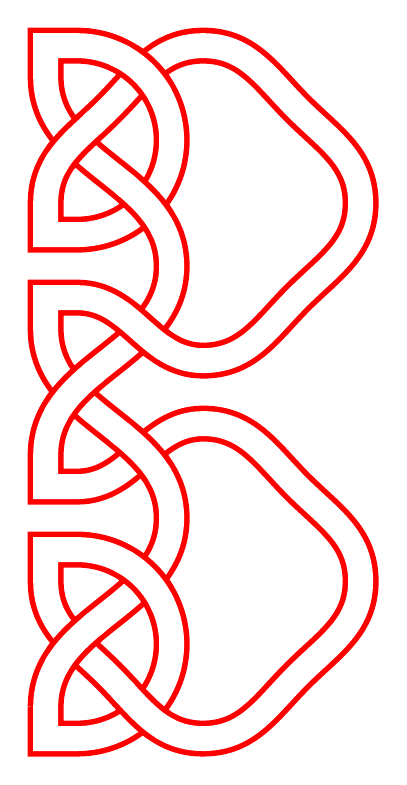
\begin{tikzpicture}[scale=0.8]

\begin{knot}[
%  draft mode=crossings,
  consider self intersections=no splits,
        end tolerance=1pt,%
        line width=2pt ,%
        line join=round,%
        clip width=1,%
        ignore endpoint intersections=true,%
        background color=red,%
        every intersection/.style={
          crossing strand
        },
        only when rendering/.style={
          basic strand
        },
        flip crossing/.list={2,3,6,8}
        ]

\strand (0.5,1) to [out=north, in=south] (2.5,4) to [out=north, in=south]
(0.5,7) -- (0.5,7) -- (0.5,7.5) -- (1,7.5) to [out=east, in=west] (3,6.5)
to [out=east, in=225] (4.5,7.5) to [out=45, in=south] (5.5,9) to
[out=north, in=-45] (4.5,10.5) to [out=135,in=east] (3,11.5) to [out=west,
in=45] (1.5,10.5) to [out=225,in=north] (0.5,9) -- (0.5,8.5) -- (1,8.5) to
[out=east, in=south] (2.5,10) to [out=north, in=east](1,11.5) --
(0.5,11.5) -- (0.5,11) to [out=south, in=north] (2.5,8) to [out=south,
in=north] (0.5,5) -- (0.5,4.5) -- (1,4.5) to [out=east, in=west] (3,5.5)
to [out=east, in=135] (4.5,4.5) to [out=-45, in=north] (5.5,3) to
[out=south, in=45] (4.5,1.5) to [out=225, in=east] (3,0.5) to [out=west,
in=-45] (1.5,1.5) to [out=135, in=south] (0.5,3) -- (0.5,3.5) -- (1,3.5)
to [out=east, in=north] (2.5,2) to [out=south, in=east] (1,0.5) --
(0.5,0.5) -- (0.5,1);
\end{knot}

\end{tikzpicture}
\end{document}
